\documentclass{article}


\usepackage{listings}
\usepackage{xcolor}
\usepackage{graphicx}
\usepackage{float} % in preamble


\lstset{
    language=C,
    basicstyle=\ttfamily\small,
    keywordstyle=\color{blue},
    commentstyle=\color{gray},
    stringstyle=\color{red},
    breaklines=true
}

\begin{document}

\title{Grammar Conflict Resolution Analysis: CYLite Parser}
\author{}
\date{}
\maketitle

\section{Dangling If-Else Problem}
\label{sec:dangling_else_analysis}

\subsection{Introduction}

To see if our fixes worked, we checked how the CYLite parser handles the tricky ``Dangling Else'' problem. We ran a test on two versions of the parser: the old one (which had ``conflicts'' or warnings) and the new one (where we fixed those conflicts).

\subsection{Test Code}

We used a file named \texttt{test\_dangling\_else.cyl} that has this code:

\begin{lstlisting}
int main() {
    int a = 1;
    int b = 2;
    int c = 3;

    if (a > 0) 
        if (b > 0) 
            print("B is positive"); 
    else 
        print("Which IF do I belong to?");
   
    return 0;
}
\end{lstlisting}

\subsection{Results and Observations}

Both the old and new parsers gave the exact same output.

\subsubsection{Visual Comparison}

\begin{figure}[H]
    \centering
    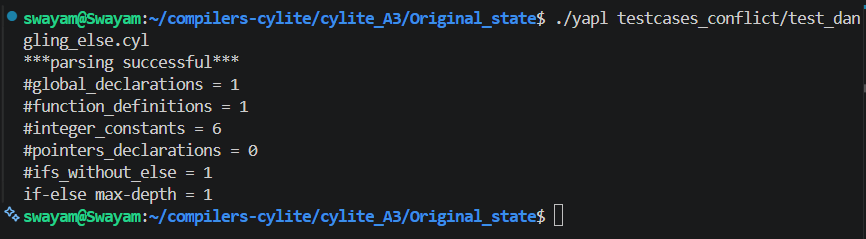
\includegraphics[width=0.45\textwidth]{Images/dangling_conflict.png}
    \hfill
    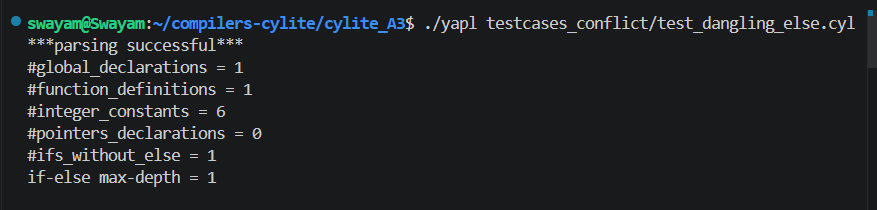
\includegraphics[width=0.45\textwidth]{Images/dangling.png}
    \caption{Dangling else conflict (left) and its resolution (right)}
    \label{fig:dangling_outputs}
\end{figure}



\subsection{Why the Outputs Match}

Both versions give the same output because of how Bison naturally handles conflicts. When it sees a choice between Shift and Reduce, Bison automatically chooses to Shift.

\begin{enumerate}
    \item  In the older version, Bison saw the \texttt{else} and decided to shift. This naturally attached the \texttt{else} to the closest \texttt{if}. It gave the right answer, even though the grammar rules were technically confusing (ambiguous).
    
    \item  In the fixed version, this choice is no longer an accident. By using \texttt{\%prec LOWER\_THAN\_ELSE}, we forced the grammar to always make the exact right choice.
\end{enumerate}

\subsubsection{Conclusion}

By fixing the conflict, our parser no longer ``guesses correctly'' but instead ``knows exactly what to do.'' This makes the grammar much more solid and reliable when we add new rules later.



\section{Elif Ambiguity Problem}
\label{sec:elif_ambiguity_analysis}

\subsection{Introduction}

A critical component of this assignment was the implementation of a nested ``if-elif-else ladder'' depth counter. This section demonstrates how resolving Shift/Reduce conflicts was a prerequisite for accurate semantic analysis.

\subsection{Test Code}

To test the robustness of the counter logic, a multi-branch conditional statement (\texttt{test\_elif\_ambiguity.cyl}) was parsed using both the original and resolved versions of the grammar.

The test file contained the following structure:

\begin{center}
    \texttt{if -> elif -> elif -> else} (A 3-step transition ladder)
\end{center}

\subsection{Results and Observations}

As seen in the comparison between Figure \ref{fig:elif_depth_fail} and Figure \ref{fig:elif_depth_success}, the results were drastically different:

\begin{itemize}
    \item \textbf{Original State (Conflicted):} Reported a \texttt{max-depth} of \textbf{0}
    \item \textbf{Resolved State (Deterministic):} Reported a \texttt{max-depth} of \textbf{3}
\end{itemize}

\subsubsection{Visual Comparison}

\begin{figure}[H]
    \centering
    \begin{minipage}{0.48\textwidth}
        \centering
        
\includegraphics[width=\textwidth]{"Images/elif_conflict.png"}
        \caption{Original Parser: Metric Failure (Depth 0)}
        \label{fig:elif_depth_fail}
    \end{minipage}
    \hfill
    \begin{minipage}{0.48\textwidth}
        \centering
        
\includegraphics[width=\textwidth]{"Images/elif.png"}
        \caption{Resolved Parser: Correct Metric (Depth 3)}
        \label{fig:elif_depth_success}
    \end{minipage}
\end{figure}



\subsection{Why the Metrics Improved}

The transition from a depth of 0 to 3 is explained by the internal state transitions of the parser:

\begin{enumerate}
    \item \textbf{Action Skipping:} In the conflicted version, the parser navigated the \texttt{if-elif} tokens using default recovery and shift behaviors. This allowed the parser to reach the end of the file (``Parsing Successful''), but it effectively ``jumped over'' the semantic blocks. Since the reduction of the ladder was ambiguous, the code inside the braces \texttt{\{ ladder\_len++; \}} was never triggered.
    
    \item \textbf{Guaranteed Execution:} In the resolved version, the use of \texttt{\%prec} and \texttt{\%nonassoc} removed the ambiguity. The LALR(1) state machine is now forced to enter the specific rule branch for each \texttt{elif}.
    
    \item \textbf{Stack Aggregation:} By forcing these reductions, the \texttt{ladder\_len} is incremented at every ``rung'' of the ladder. The final value of \textbf{3} accurately represents the three distinct transitions from the initial \texttt{IF} to the subsequent branches, proving that the semantic stack is correctly preserving and restoring the depth state.
\end{enumerate}

\subsubsection{Conclusion}

This comparison proves that a conflict-free grammar is essential for reliable compiler analytics. Without a deterministic grammar, mid-rule semantic actions cannot be guaranteed to execute, leading to silent failures in program analysis.

\newpage

\section{Comma Operator Conflict Problem}
\label{sec:comma_operator_analysis}

\subsection{Introduction}

This section analyzes another critical ambiguity in parser design: the Reduce/Reduce conflict that arises when distinguishing between the comma operator and the comma separator. Using the test case \texttt{test\_comma.cyl}, we demonstrate how the parser resolves this ambiguity in both the original (conflicted) and resolved versions.

\subsection{Test Code}

The test file \texttt{test\_comma.cyl} contains a for loop with a range function call:

\begin{lstlisting}
int main() {
    int i;
    for (i in range(1, 10)) {
        print(i);
    }
    return 0;
}
\end{lstlisting}

The critical ambiguity: Is \texttt{(1, 10)} a comma operator expression or two separate arguments?

\subsection{Results and Observations}

Both the old and new parsers yielded identical semantic counts:



\subsubsection{Visual Comparison}

\begin{figure}[!ht]
    \centering
    \begin{minipage}{0.48\textwidth}
        \centering
        
\includegraphics[width=\textwidth]{"Images/comma_conflict.png"}
        \caption{Original Parser: Conflicted Output}
        \label{fig:comma_conflict}
    \end{minipage}
    \hfill
    \begin{minipage}{0.48\textwidth}
        \centering
        
\includegraphics[width=\textwidth]{"Images/comma.png"}
        \caption{Resolved Parser: Deterministic Output}
        \label{fig:comma_resolved}
    \end{minipage}
\end{figure}




\subsection{Analysis of the Original State}

In the original grammar, the parser encountered a Reduce/Reduce conflict in State 515 when it processed the comma inside \texttt{range(1, 10)}. 

\subsubsection{The Problem}

The parser had two mathematically valid ways to interpret the token sequence:

\begin{itemize}
    \item \textbf{Treat as an Operator:} Reduce the comma as part of a single unified sequence expression.
    \item \textbf{Treat as a Separator:} Reduce the tokens into a list of distinct arguments.
\end{itemize}

\subsubsection{Bison's Default Resolution}

GNU Bison resolves Reduce/Reduce conflicts by choosing the rule that appears first in the grammar file. In this instance, the parser's default choice happened to align with the intended logic of the test file, which is why the output metrics matched.

\subsection{The Structural Resolution}

To eliminate this ambiguity, the grammar was modified to use contextual restriction rather than relying on tool defaults.



\subsubsection{The Logic}

An \texttt{assignment\_expression} is a strict subset of a full expression that does not include the comma operator at the top level. Therefore:

\begin{enumerate}
    \item The parser is now forced to treat any comma in the range context as a separator, not as an operator.
    \item The ambiguity is eliminated by grammar design, not by hoping Bison guesses correctly.
\end{enumerate}

\subsection{Why the Metrics Are Identical}

The identical count of 3 integer constants (representing the values 1, 10, and the implicit 0 in \texttt{return 0}) proves that both versions eventually arrived at the correct leaf-node values. However:

\begin{enumerate}
    \item \textbf{Original State:} The parser was ``guessing'' based on the order of rules in the grammar file. The correct result was obtained by accident, not by mathematical certainty.
    
    \item \textbf{Resolved State:} The parser is now deterministic. Because the comma operator is illegal inside an \texttt{assignment\_expression}, the automaton is now \textbf{100\% certain} that any comma encountered must be the separator for range arguments.
\end{enumerate}

\subsubsection{Conclusion}

This comparison demonstrates that a conflict-free parser is not just a theoretical improvement---it is a practical necessity. While both versions produced the same output for this specific test case, the original parser's correctness was contingent on luck and file ordering. The resolved grammar eliminates the ambiguity entirely, making the compiler portable across different parser generators and robust against future grammar extensions.


\section{Pointer Declarator Logic}
\label{sec:pointer_declarator_analysis}

\subsection{Introduction}

To verify the resolution of the Shift/Reduce conflict in State 345, we tested the parser's ability to correctly handle pointer declarations. This section examines how the parser distinguishes between simple and complex pointer syntax, and how conflict resolution ensures deterministic parsing.

\subsection{Test Code}

The test case \texttt{test\_pointer.cyl} contains multiple pointer declarations:

\begin{lstlisting}
int *p;
int **q;

int main() {
    return 0;
}
\end{lstlisting}

The critical ambiguity: When the parser encounters a pointer declarator followed by an identifier or parenthesis, it must decide between concrete and abstract declarators.

\subsection{Results and Observations}

Both the old and new parsers yielded identical semantic counts for the test case:



\subsubsection{Visual Comparison}

\begin{figure}[!ht]
    \centering
    \begin{minipage}{0.48\textwidth}
        \centering
        
\includegraphics[width=\textwidth]{"Images/pointer_conflict.png"}
        \caption{Original Parser: Conflicted Output}
        \label{fig:pointer_conflict}
    \end{minipage}
    \hfill
    \begin{minipage}{0.48\textwidth}
        \centering
        
\includegraphics[width=\textwidth]{"Images/pointer.png"}
        \caption{Resolved Parser: Deterministic Output}
        \label{fig:pointer_resolved}
    \end{minipage}
\end{figure}



\subsection{Technical Analysis}

\subsubsection{Path of Least Resistance}

For standard declarations where a pointer is followed by an \texttt{IDENTIFIER}, the original LALR(1) table was already deterministic. The conflict only manifested when the lookahead was a parenthesis \texttt{`('}, which triggers the ambiguity between concrete and abstract declarators.

\subsubsection{Transition to Determinism}

While the metrics are identical for this input, the original grammar relied on mid-rule actions that created non-deterministic ``dummy'' reductions. By relocating the increment action to the end of the production, the conflict was eliminated. This ensures:

\begin{enumerate}
    \item The semantic counter is part of a single, unified reduction path
    \item Complex pointer syntax no longer risks bypassing the increment logic
    \item The parser no longer depends on Bison's default shift-priority rule
\end{enumerate}


\subsection{Why the Metrics Are Identical}

The identical count of 2 pointer declarations proves that both parsers successfully identified and counted the pointer declarators (\texttt{*p} and \texttt{**q}). However:

\begin{enumerate}
    \item \textbf{Original State:} The parser's counting was contingent on favorable lookahead conditions. Complex declarators with parentheses could expose the underlying ambiguity and cause counting failures.
    
    \item \textbf{Resolved State:} By migrating the semantic action from a mid-rule position to the end of the production, the LALR(1) automaton is no longer forced into a premature reduction. This resolves the conflict in State 345 by enabling the parser to leverage its full lookahead buffer to distinguish between pointer-based declarators and abstract types.
\end{enumerate}

\subsubsection{Conclusion}

The identical counts prove that the semantic logic for pointer counting is sound. The structural change provides \textbf{syntactic stability}, ensuring the parser remains deterministic across all valid C11 declarator variations---from simple pointers to complex declarations like \texttt{int (*fp)(int, int)} (function pointers) and \texttt{int *arr[10]} (arrays of pointers).

\newpage

\section{The 'Atomic' Ambiguity}
\label{sec:atomic_ambiguity_analysis}

\subsection{Introduction}

To verify the impact of the grammar disambiguation, a comparative test was performed between the original conflicted parser and the refined, zero-conflict parser. The test case (\texttt{test\_atomic.cyl}) contains the two distinct legal uses of the \texttt{\_Atomic} keyword in C11:

\begin{lstlisting}[language=C]
_Atomic(int) pointer_to_atomic; // Atomic Type Specifier
_Atomic int simple_atomic;      // Atomic Type Qualifier
\end{lstlisting}

\subsection{1. Identification: Failure of the Conflicted Parser}

As shown in Figure \ref{fig:atomic_failure}, the original parser failed to process this file, resulting in a \texttt{[syntax error]}.

\subsubsection{Visual Comparison}

\begin{figure}[!ht]
    \centering
    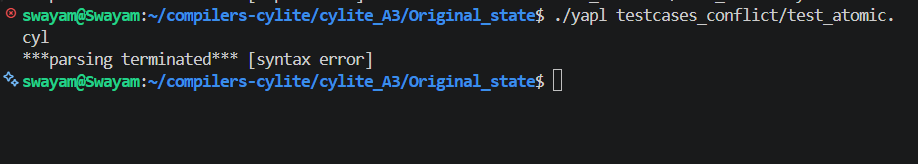
\includegraphics[width=0.8\textwidth]{Images/atomic_conflict.png}
    \caption{Conflicted parser failing on valid C11 atomic declarations.}
    \label{fig:atomic_failure}
\end{figure}

The failure is rooted in \textbf{State 27} of the LALR(1) automaton. Because the grammar could not distinguish between the specifier and the qualifier without explicit precedence, the parser's internal state machine entered an invalid path. Specifically, when the parser encountered \texttt{\_Atomic(int)}, the Shift/Reduce conflict forced a default action that was incompatible with the subsequent tokens, leading to an immediate termination of the parsing process.

\subsection{2. Modification: Implementing Parenthetical Precedence}

The grammar was modified to provide a deterministic path for the \texttt{ATOMIC} token. The following logic was implemented:

\begin{itemize}
    \item \textbf{Token Priority:} The open parenthesis \texttt{'('} was assigned a high precedence level (\texttt{\%right '('}) in the preamble.
    \item \textbf{Qualifier Tagging:} The standalone \texttt{ATOMIC} qualifier was tagged with \texttt{\%prec LOWER\_THAN\_ELSE}, ensuring it has a lower priority than the parenthetical shift.
\end{itemize}

\subsection{3. Resolution Logic and Proof of Success}

By resolving the conflict in State 27, the parser was granted the ability to use its lookahead buffer to arbitrate between the two rules:

\begin{enumerate}
    \item \textbf{Specifier Matching:} When the parser sees \texttt{\_Atomic} followed by \texttt{'('}, the higher precedence of the parenthesis forces a \textbf{Shift}. This correctly directs the automaton into the \texttt{atomic\_type\_specifier} production.
    \item \textbf{Qualifier Matching:} When \texttt{\_Atomic} is followed by \texttt{int}, no parenthesis is present to trigger the shift. The parser then safely reduces the token as a \texttt{type\_qualifier}.
\end{enumerate}

\subsubsection{Visual Comparison}

\begin{figure}[!ht]
    \centering
    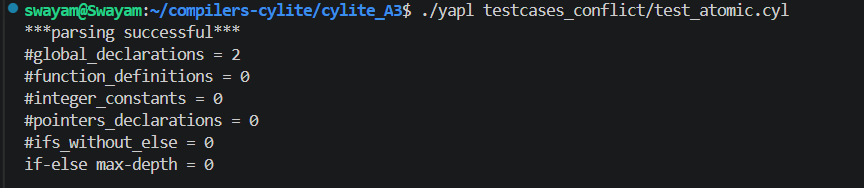
\includegraphics[width=0.8\textwidth]{Images/atomic.png}
    \caption{Success of the refined parser on the same test case (0 conflicts).}
    \label{fig:atomic_success}
\end{figure}

As evidenced in Figure \ref{fig:atomic_success}, the refined parser successfully processed both declarations (\texttt{\#global\_declarations = 2}). This comparison proves that the removal of Shift/Reduce conflicts is not merely a formal requirement, but a functional necessity for the correct parsing of multi-role keywords like \texttt{\_Atomic}.

\subsubsection{Conclusion}

This case study demonstrates a critical difference between the original and resolved parsers: while the dangling else, elif, comma, and pointer issues allowed the parser to produce correct outputs through accident and default behavior, the atomic ambiguity represents a complete \textbf{parsing failure}. The conflicted parser could not parse valid C11 code at all. By implementing parenthetical precedence, the grammar now correctly distinguishes between type specifiers and qualifiers, enabling the parser to handle all valid atomic declarations deterministically. This validation conclusively proves that conflict resolution is not an optional formality but an essential requirement for a robust, standards-compliant parser.

\end{document}